
\documentclass[10pt,a4paper]{article}
\usepackage[T1]{fontenc}
\usepackage{tikz}
\usepackage[margin=1cm]{geometry}
\begin{document}

\section*{Final Binary Search Tree}
This document presents the final binary search tree generated through the user-driven node insertion process. The binary tree structure is designed to start from a root node and grows as new nodes are inserted based on user input. The following sections detail the algorithm and the visualization of the tree.

\subsection*{Tree Construction Process}
The binary tree was constructed using the following steps:
\begin{enumerate}
    \item \textbf{Insertion of Root Node:} The process begins by inserting the root node, which serves as the starting point of the tree.
    \item \textbf{Adding Child Nodes:} Subsequent nodes are added by comparing them with existing nodes. If the new node�s value is less than the current node's value, it is placed in the left subtree; otherwise, it goes to the right subtree.
    \item \textbf{Recursive Structure:} The tree maintains a recursive structure, where each node can have up to two children (left and right). Each insertion involves traversing the tree recursively until the appropriate position for the new node is found.
\end{enumerate}

\subsection*{Final Tree Visualization}
The final binary tree is visualized below:

\begin{center}
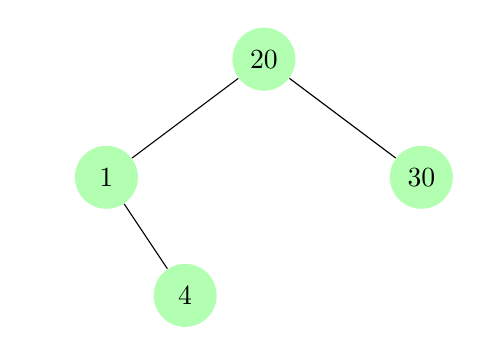
\begin{tikzpicture}[level distance=15mm, sibling distance=20mm]
    \tikzstyle{every node}=[fill=green!30,circle,inner sep=1pt, minimum size=8mm]
    \tikzstyle{level 1}=[sibling distance=40mm, set style={{every node}+=[fill=green!30]}]
    \tikzstyle{level 2}=[sibling distance=20mm, set style={{every node}+=[fill=green!30]}]
    \tikzstyle{level 3}=[sibling distance=15mm, set style={{every node}+=[fill=green!30]}]
    \tikzstyle{level 4}=[sibling distance=10mm, set style={{every node}+=[fill=green!30]}]

% The following code generates the final binary search tree (BST) after all insertions.

    \node {20} child {node {1} child[fill=none] {edge from parent[draw=none]} child {node {4} }} child {node {30} };

\end{tikzpicture}
\end{center}

\end{document}
